\chapter{Métodos}

Neste capitulo percorremos as experiências realizadas. Estas foram feitas atraves do usos do programas criados para o efeito, disponiveis no repositorio GitHub do \href{https://github.com/JotaFan/renewable-generation-into-reserve-markets}{projecto}.

\section{Benchmark}

Como modelo bencharmark iremos usar a alocação feita. Pois são estes valores que procuramos melhorar no caso prático.



\begin{figure}[H]
    \centering
    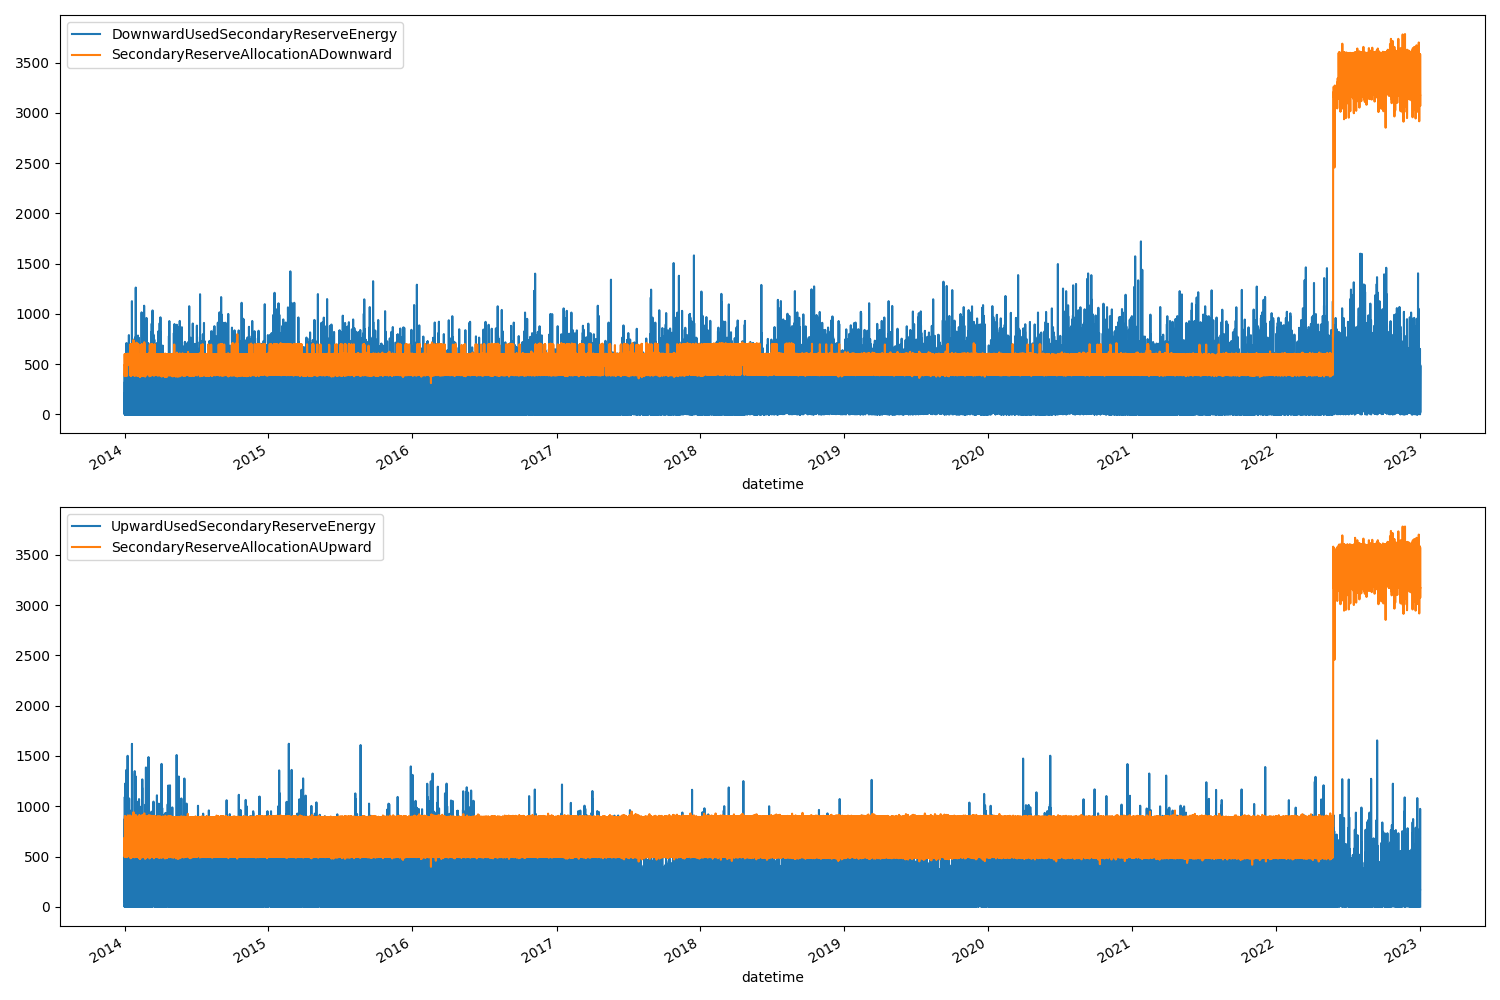
\includegraphics[width=0.8\textwidth]{../plots/benchmark.png}
    \caption{Serie Temporal do benchmark}
    \label{fig:benchmark}
\end{figure}
  

\resizebox{\linewidth}{!}{\csvautotabular{../data/benchmark_scores.csv}  \label{tb:benchmark}}

Para validação dos mesmo, vamos usar o ano 2021, devido aquele salto nos valores de alocação em 2022.

Para esses temos os seguintes dados:

\begin{figure}[H]
    \centering
    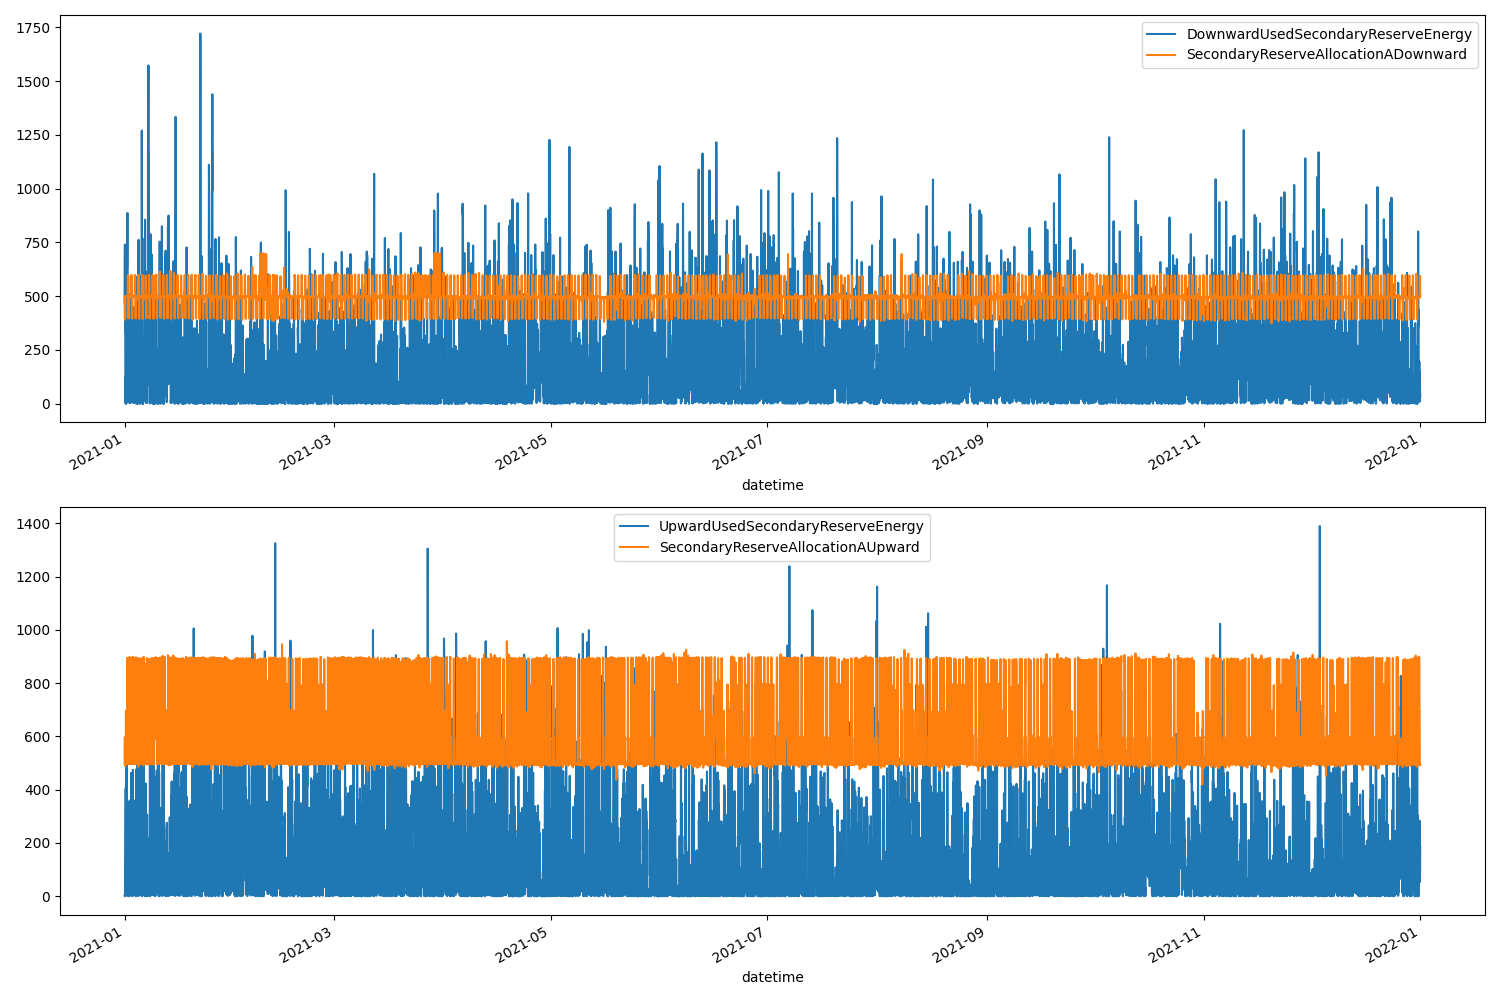
\includegraphics[width=0.8\textwidth]{../plots/benchmark_validation.png}
    \caption{Serie Temporal do benchmark 2021}
    \label{fig:benchmark_validation}
\end{figure}
  

Os metodos em estudo vão ser comparados a esta medida. Sendo que o principal é baixar tanto a alocação perdida, como a alocação a mais. Que se traduzem no erro absoluto.

\resizebox{\linewidth}{!}{\csvautotabular{../data/benchmark_validation_scores.csv}  \label{tb:benchmark_val}}


\section{Modelos estatiscos  \label{se:model_stats}}

Antes de entrar para o densenvolvimento de modelos vamos usar metódos e modelos abertos para usar comparativamente.
Para as equações apresentadas temos que \textit{$Y_t$} é a variavel alvo, no tempo \textit{t}

Os modelos estatiscos recurrentes em previsões são AR, MA, ARMA, ARIMA, SARIMA para previsões so com um atributo, e para multiplos atributos VAR.

O modelo AR não teve resultados aplicaveis, logo foi desconsiderado.




\subsection{MA}

AR eé blabla

\begin{equation} \label{eq:MA} 
    Y_t = c + \theta_1 \varepsilon_{t-1} + \theta_2 \varepsilon_{t-2} + \dots + \theta_q \varepsilon_{t-q} + \varepsilon_t 
\end{equation}

\begin{figure}[H]
    \centering
    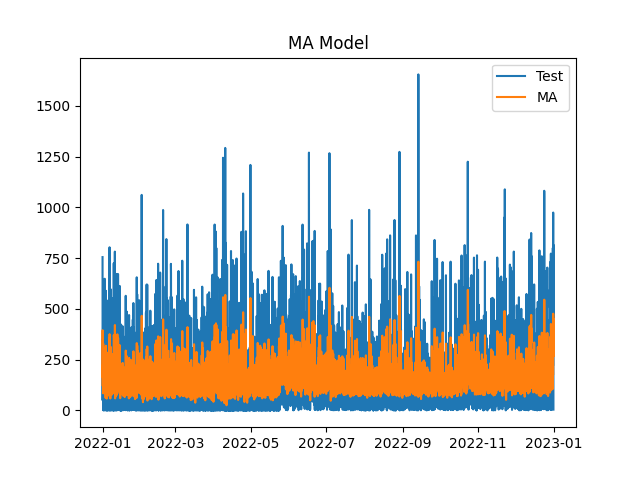
\includegraphics[width=0.8\textwidth]{../plots/MA_model.png}
    \caption{Previsões 2021 com modelo MA}
    \label{fig:MA_model}
\end{figure}
  
\subsection{ARMA}

AR eé blabla

\begin{equation} \label{eq:ARMA}  Y_t = c + \phi_1 Y_{t-1} + \phi_2 Y_{t-2} + \dots + \phi_p Y_{t-p} + \theta_1 \varepsilon_{t-1} + \theta_2 \varepsilon_{t-2} + \dots + \theta_q \varepsilon_{t-q} + \varepsilon_t  \end{equation}

\begin{figure}[H]
    \centering
    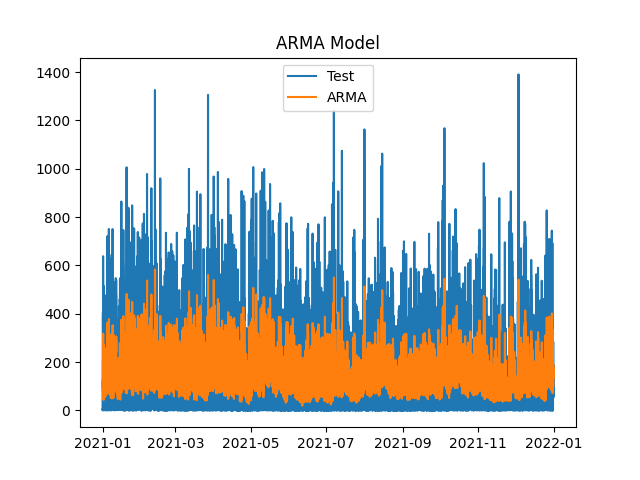
\includegraphics[width=0.8\textwidth]{../plots/ARMA_model.png}
    \caption{Previsões 2021 com modelo ARMA}
    \label{fig:ARMA_model}
\end{figure}

\subsection{ARIMA}

AR eé blabla

\begin{equation} \label{eq:ARIMA} Y't = c + \phi_1 Y'{t-1} + \phi_2 Y'{t-2} + \dots + \phi_p Y'{t-p} + \theta_1 \varepsilon_{t-1} + \theta_2 \varepsilon_{t-2} + \dots + \theta_q \varepsilon_{t-q} + \varepsilon_t \end{equation}

\begin{figure}[H]
    \centering
    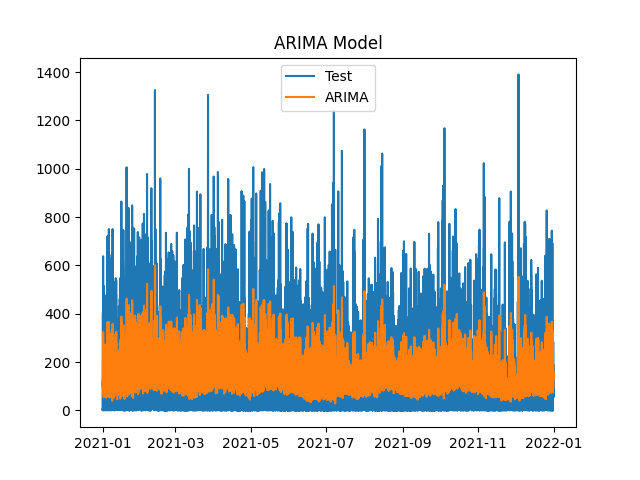
\includegraphics[width=0.8\textwidth]{../plots/ARIMA_model.png}
    \caption{Previsões 2021 com modelo ARIMA}
    \label{fig:ARIMA_model}
\end{figure}

\subsection{SARIMA}

AR eé blabla

\begin{equation} \label{eq:SARIMA} Y_t = c + \phi_1 Y_{t-1} + \phi_2 Y_{t-2} + \dots + \phi_p Y_{t-p} + \theta_1 \varepsilon_{t-1} + \theta_2 \varepsilon_{t-2} + \dots + \theta_q \varepsilon_{t-q} + \varepsilon_t \end{equation}

\begin{figure}[H]
    \centering
    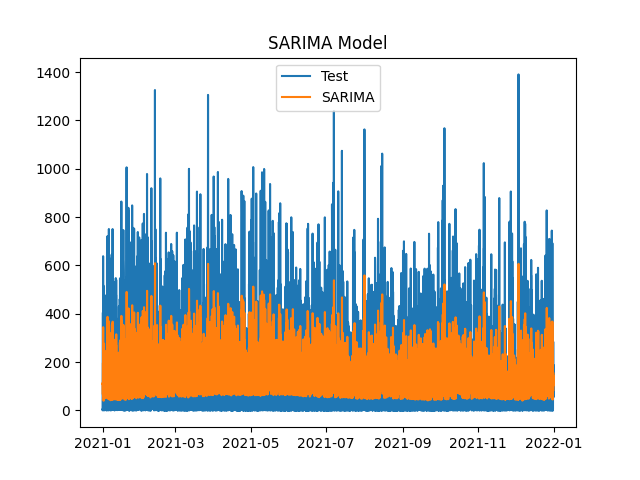
\includegraphics[width=0.8\textwidth]{../plots/SARIMA_model.png}
    \caption{Previsões 2021 com modelo SARIMA}
    \label{fig:SARIMA_model}
\end{figure}

\resizebox{\linewidth}{!}{\begin{tabular}{llllllllll}
\toprule
rmse & abs erro & erro comp & r2 score & mape score & alloc missing & alloc surplus & optimal percentage & better allocation & beter percentage \\
\midrule
NaN & 0.00 & True & -0.65 & NaN & NaN & NaN & 0.00 & 0.00 & 0.00 \\
171.14 & 1123214.13 & True & 0.14 & 17.04 & 560507.02 & 562707.11 & 63.79 & 63.79 & 86.84 \\
169.99 & 1108555.94 & True & 0.15 & 16.36 & 554443.34 & 554112.60 & 64.04 & 64.04 & 87.17 \\
170.13 & 1111215.12 & True & 0.15 & 16.52 & 556281.62 & 554933.50 & 64.03 & 64.03 & 87.01 \\
171.88 & 1115725.36 & True & 0.13 & 16.43 & 568538.03 & 547187.33 & 63.45 & 63.45 & 86.92 \\
184.60 & 1253196.02 & True & -0.00 & 21.63 & 619929.79 & 633266.23 & 64.82 & 64.82 & 86.07 \\
\bottomrule
\end{tabular}
} %\label{tb:statitics_scores}


Apenas pelos métodos estatisticos verificamos que no ano de 2021 teria havido uma melhoria de cerca de 80\% das vezes, usando qualquer um dos métodos apresentados.
Embora a alocação em falta seja de uma ordem de grandeza superior.


\section{Forecat  \label{se:forecat}}


Com o propósito de desenvolver este estudo, e deixar ferramentas para a replicação do mesmo, foi criado uma biblioteca em python para desenhar as arquitecturas em estudo.
TODO: url

\subsection{Construtor de modelos}

Esta ferramenta 

\subsection{subsubsection Gerador de dados (depth 2)}
distribuição

clustering


\section{Treino e Resultados  \label{se:training}}

Realizaram-se várias experiências, onde em cada um se ia elimando alguns dos objectos em estudo.
Em casa experiências toda a parametrização era igual, à excepção do objecto de estudo.

\subsection{Arquiteturas e numeros de epocas}

Nesta experiência foi testado o resultado das várias arquiteturas em estudo, como também o impacto do numero de epocas na qualidade dos modelos-
As arquitecturas estudadas foram:

%TODO: arranjar reseach para cada uma 

\begin{itemize}
    \item[--] VanillaDense
    \item[--] VanillaCNN
    \item[--] VanillaLSTM
    \item[--] StackedCNN
    \item[--] StackedLSTM
    \item[--] EncoderDecoder
    \item[--] UNET
\end{itemize}

O modelos foram treinados em 200 epocas, sendo que foram salvos a cada 10 epocas, de forma conseguirmos perceber os contextos nos saltos de epocas.

As parametrizações usadas:
\begin{itemize}
    \item[--] loss : mean squared error
    \item[--] Metodo activação no meio : relu
    \item[--] Metodo activação no fim : relu
    \item[--] optimizador : Adam
    \item[--] Janela temporal em X : 168 horas (1 semana)
    \item[--] Janela temporal em Y : 24 horas (1 semana)
    \item[--] Fracção de treino : 95%  
\end{itemize}

\subsection{Funções de Perda (Loss)}

TODO: o que é a loss function?

Esta experiência consiste em rever que função de perda é melhor aplicavel ao problema. Sendo um problema de regressao linear, de valores bastante oscilatórios e com uma distribuição exponencial, temos algumas loss functions que já são reconhecidas para o problema.

\begin{itemize}
    \item[--] mean absolute error
    \item[--] mean squared error    
    \item[--] loss : mean absolute error

\end{itemize}



\subsection{Hiperparametrização}

\subsubsection{Activação}

\subsubsection{Optimizadores}

\subsection{Janelas Temporais}

Um dos pontos deste trabalho é perceber a fesiabilidade de usar dados de previsão do dia anterior (DA) para estes atributos energéticos.
Algo que pode ser também aplicado no futuro a outros dados que não DA, mas sim a 3 horas, ou a 8 horas.
Para perceber esta flexibilidade, mas especialmente para escolher as melhores janelas temporais a usar neste modelos, vamos testar várias combinações.
Mantendo em mente que o objectivo é prever 24 horas, para os casos onde o alvo não dá um previsão de 24 horas, é necessario criar um numero de modelos para fazer as 24 horas.
Para validação apenas é usado o espaço temporar previsto, e não multiplos modelos.

Dado as análises de autocorrelação iremos usar como janelas para treino o conjunto [24, 48, 98, 168] para prever o conjunto [1, 4, 8, 12, 24]


Para alem destes foram também testadas combinações com janelas de treino 8 e 12 horas. Estas mostraram rapidamente que janelas de treino menores que as de previsão funcionam muito mal.

\subsection{Classificação}

Como descrito em (ref)... existe também o uso de tanto classes como valores linears para resoluçao de problemas de regressão, também chamado \textit{cluster-wise regression}.
Para este teste mudamos um pouco o modelo em uso. Ao invés de apenas uma camada interpretativa, fazemos duas, em paralelo, sendo que uma resolve a regressão e a outra a classificação.
Outro caso, proposto aqui, é usar uma nova camada intrepertativa, que combina as duas saidas anteriores (linear e classificação), e resolve novamente para os valores lineares.

Estes modelos não teram apenas uma saida, mas varias, como as arquiteturas MultiTail, mas neste caso cada uma resolve para um problema diferente, com funções de perda, e activações diferentes.

TODO: desenho destas duas camadas intrepretaticas

\subsection{Pesos}

Por ultimo foi testado o impacto do uso de pesos nos modelos. Estes pesos são o peso que aquele alvo TODO: epxlicar pesos

\subsubsection{Modelos lineares}

Para os modelos lineares o peso que é adiciona ao modelo é a distância à média.
Este peso serve para dar mais importância a valores facilmente considerados outliers.



\subsubsection{Modelos Lineares e de Classificação}
Aqui o peso é dado por saida. Para as saidas lineares o peso dados é o mesmo que apresentado anteriormente, para a saida de classificaçao, o peso é o inverso da frequência da classe.
Distribuindo assim a importância de treino pela frquência das classes. Sendo um prática comum especialmente quando as distribuiçoes são muito desiguais, como o caso em estudo.
É aqui estudada a aplicaçao destes pesos individualmente, e em conjunto. 
Os pesos aqui são tambem normalizados de modo a que o maior peso em cada um deles seja 1, e logo a multiplicaçao dos dois esteja dentro das mesmas dimensões de relevância.


\begin{equation} \label{eq:peso_media} 
    P_m = \left| y - mean \right| 
\end{equation}

\section{Considerações adicionais  \label{se:metodos_plus}}

Foram realizados testes adicionais que não obtiveram resultados passivos de boa interpretação, e foram imediatamente descartados, como:

\begin{itemize}
    \item[--] Janela temporal em X : 96, 48, 24
    \item[--] optimizador : todos os optimizadores disponiveis na biblioteca keras
    \item[--] loss : todas as outra loss functions de regressão disponiveis.
    \item[--] epocas : influência do numero de epocas nos modelos, foram treinados até 20000 epocas alguns modelos mas à medida que a perda ia estagnando na assintomta, o modelo ia apenas piorando.
\end{itemize}


Todos os metodos foram realizados utilizando código em python, que está aberto em https://github.com/JotaFan/renewable-generation-into-reserve-markets
